\documentclass[border=20pt]{standalone}
\usepackage{tikz}
\usetikzlibrary{arrows.meta, positioning, fit, backgrounds}

\begin{document}
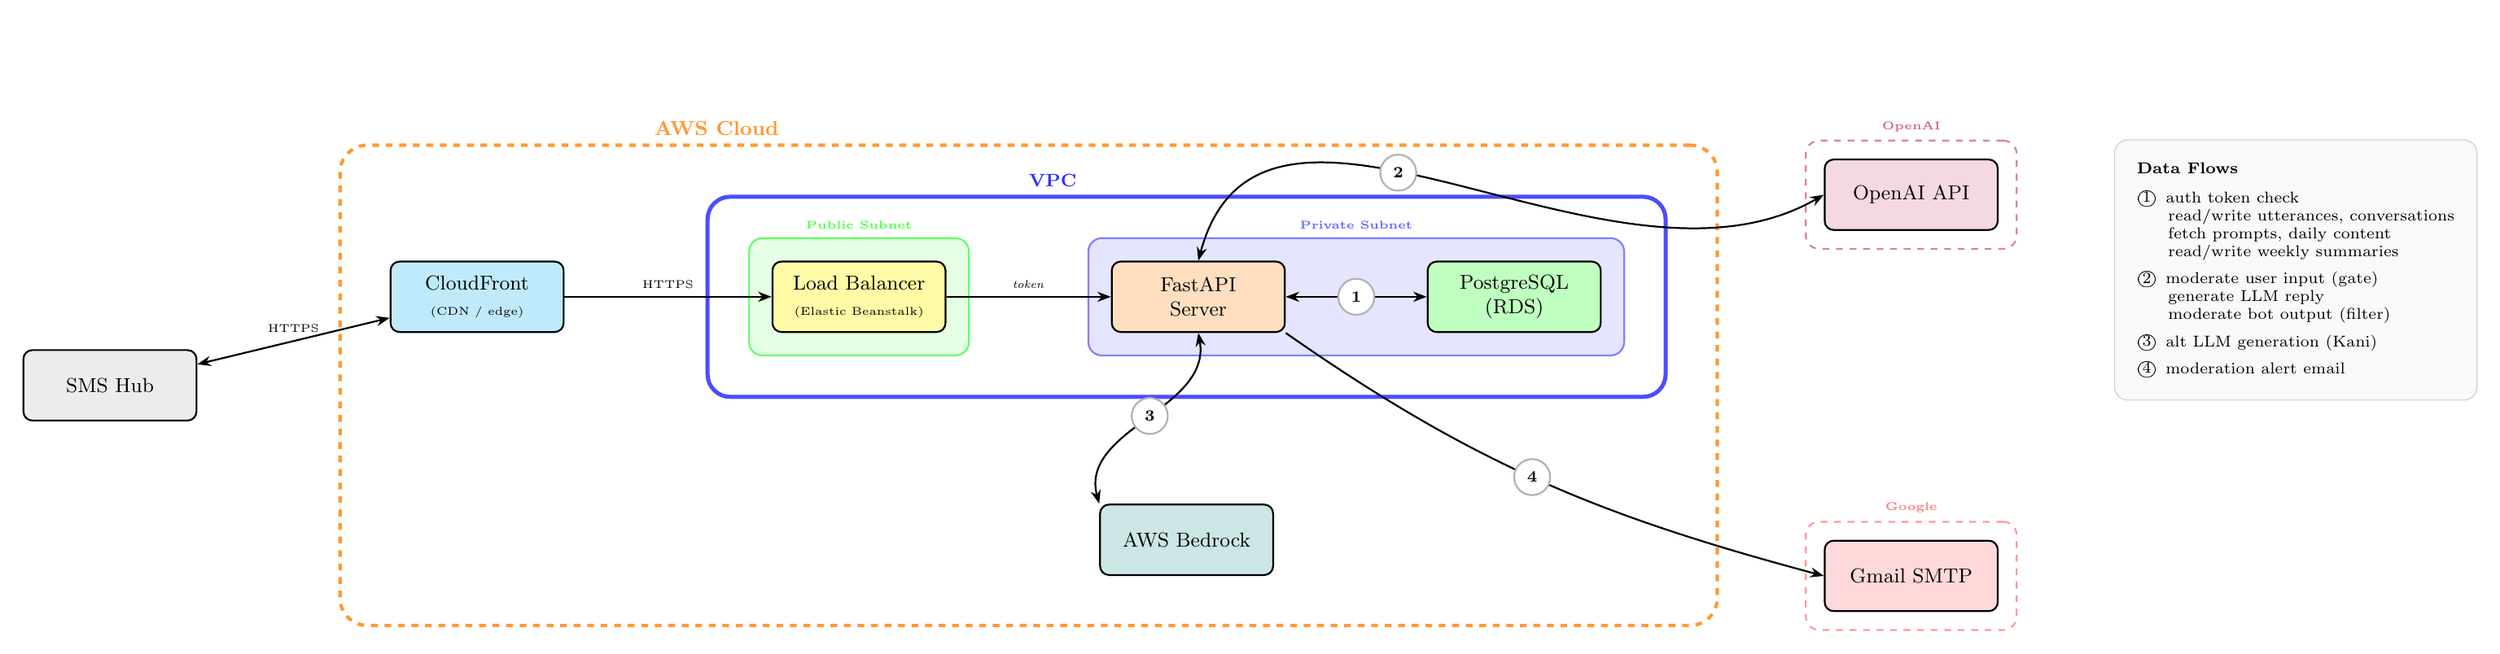
\begin{tikzpicture}[
  component/.style={
    rectangle, rounded corners=4pt,
    minimum width=2.7cm, minimum height=1.1cm,
    draw, thick, align=center, font=\small
  },
  cloudbound/.style={
    rectangle, rounded corners=12pt,
    draw=orange!80, line width=1.5pt, dashed, fill=none, inner sep=22pt
  },
  vpcbound/.style={
    rectangle, rounded corners=10pt,
    draw=blue!70, line width=1.8pt, fill=none, inner sep=18pt
  },
  subnetbound/.style={
    rectangle, rounded corners=6pt,
    draw, thick, inner sep=10pt
  },
  extbound/.style={
    rectangle, rounded corners=6pt,
    draw, thick, dashed, fill=none, inner sep=8pt
  },
  arr/.style={-{Stealth[length=6pt]}, thick},
  darr/.style={{Stealth[length=6pt]}-{Stealth[length=6pt]}, thick},
  lbl/.style={font=\tiny, midway},
  num/.style={font=\scriptsize\bfseries, shape=circle, draw=gray!60,
              fill=white, inner sep=2pt, minimum size=16pt},
]

%% ════════════════════════════════════════════════
%% LAYER 1 — INFRA
%% Rule: define inside-out so fit() always has its targets.
%% No fills on VPC/AWS — avoids background-layer paint-over.
%% ════════════════════════════════════════════════

%% Private subnet
\node[component, fill=orange!25] (fastapi) {FastAPI\\Server};
\node[component, fill=green!25, right=2.2cm of fastapi] (postgres) {PostgreSQL\\(RDS)};

\begin{scope}[on background layer]
  \node[subnetbound, draw=blue!50, fill=blue!10,
        fit=(fastapi)(postgres),
        label={[text=blue!60, font=\tiny\bfseries]above:Private Subnet}] (priv) {};
\end{scope}

%% Public subnet
\node[component, fill=yellow!35, left=2.2cm of priv] (elb) {Load Balancer\\{\tiny(Elastic Beanstalk)}};

\begin{scope}[on background layer]
  \node[subnetbound, draw=green!60, fill=green!10,
        fit=(elb),
        label={[text=green!70, font=\tiny\bfseries]above:Public Subnet}] (pub) {};
\end{scope}

%% VPC — no fill so inner subnets stay visible
\begin{scope}[on background layer]
  \node[vpcbound, fit=(pub)(priv),
        label={[text=blue!80, font=\footnotesize\bfseries]above left:VPC}] (vpc) {};
\end{scope}

%% CloudFront — inside AWS, outside VPC
\node[component, fill=cyan!25, left=2.2cm of vpc] (cf) {CloudFront\\{\tiny(CDN / edge)}};

%% AWS Bedrock — inside AWS (same account), outside VPC, positioned below VPC
\node[component, fill=teal!20]
  (bedrock) at ([yshift=-2.2cm]vpc.south) {AWS Bedrock};

%% AWS Cloud — fits around cf + vpc + bedrock (Bedrock is same-account AWS service)
\begin{scope}[on background layer]
  \node[cloudbound, fit=(cf)(vpc)(bedrock),
        label={[text=orange!80, font=\small\bfseries]above left:\textbf{AWS Cloud}}] (aws) {};
\end{scope}

%% SMS Hub — left of AWS
\node[component, fill=gray!15, left=2.2cm of aws] (smshub) {SMS Hub};

%% ════════════════════════════════════════════════
%% External services — right of AWS (not AWS-owned)
%% ════════════════════════════════════════════════

\node[component, fill=purple!15]
  (openai) at ([xshift=3cm, yshift=-0.8cm]aws.north east) {OpenAI API};
\node[component, fill=red!15]
  (gmail)  at ([xshift=3cm, yshift=0.8cm]aws.south east)  {Gmail SMTP};

\begin{scope}[on background layer]
  \node[extbound, draw=purple!50, fit=(openai),
        label={[text=purple!60, font=\tiny\bfseries]above:OpenAI}] {};
  \node[extbound, draw=red!40, fit=(gmail),
        label={[text=red!50, font=\tiny\bfseries]above:Google}] {};
\end{scope}

%% ════════════════════════════════════════════════
%% CONNECTIONS
%% ════════════════════════════════════════════════

%% Infra path
\draw[darr] (smshub) -- node[lbl, above]{HTTPS} (cf);
\draw[arr]  (cf)     -- node[lbl, above]{HTTPS}  (elb);
\draw[arr]  (elb)    -- node[lbl, above]{\textit{token}} (fastapi);

%% 1 FastAPI ↔ PostgreSQL — all persistence (stays in private subnet)
\draw[darr] (fastapi) -- node[num]{1} (postgres);

%% 2 FastAPI ↔ OpenAI — moderation + LLM (exits AWS)
\draw[darr] (fastapi.north) to[out=75, in=210] node[num, pos=0.42]{2} (openai.west);

%% 3 FastAPI ↔ Bedrock — alt LLM (within AWS, exits VPC only)
\draw[darr] (fastapi.south) to[out=-80, in=105] node[num, pos=0.48]{3} (bedrock.north west);

%% 4 FastAPI → Gmail SMTP — alert email (exits AWS)
\draw[arr] (fastapi.south east) to[out=-35, in=165] node[num, pos=0.48]{4} (gmail.west);

%% ════════════════════════════════════════════════
%% LEGEND
%% ════════════════════════════════════════════════

\node[draw=gray!40, rounded corners=6pt, fill=gray!5, inner sep=10pt,
      align=left, font=\scriptsize, anchor=north west]
  at ([xshift=1.8cm, yshift=0.3cm]openai.north east) {
  \textbf{Data Flows}\\[5pt]
  \textcircled{1}\enspace auth token check\\
  \hspace{1.4em} read/write utterances, conversations\\
  \hspace{1.4em} fetch prompts, daily content\\
  \hspace{1.4em} read/write weekly summaries\\[4pt]
  \textcircled{2}\enspace moderate user input (gate)\\
  \hspace{1.4em} generate LLM reply\\
  \hspace{1.4em} moderate bot output (filter)\\[4pt]
  \textcircled{3}\enspace alt LLM generation (Kani)\\[4pt]
  \textcircled{4}\enspace moderation alert email
};

\end{tikzpicture}
\end{document}
